\title{Lecture 9: Counting Principles}

\frame{\titlepage}

\begin{frame}
\addfig{0.8}{loot_box}{The Box}
\end{frame}

%%%%%%%%%%%%%
\section[Concept]{Combinatorial concepts}
\frame{\sectionpage}
%%%%%%%%%%%%%

\begin{frame}
\frametitle{How to Count without Counting}
\addfig{0.5}{combinatorics_intro}{\href{https://brilliant.org/wiki/combinatorics/}{Combinatorics on brillant.org}}
\end{frame}

\begin{frame}
\frametitle{Keywords}
\begin{itemize}
\item How many ways to \ldots
\item Choose, select, pick, form a group
\item Arrange, order, place
\item Distinct vs. repetion
\end{itemize}
\end{frame}

%%%%%%%%%%%%%
\section{Rule of Product}
\frame{\sectionpage}
%%%%%%%%%%%%%

\begin{frame}
\frametitle{Rule of product for two arrangements}
\begin{thm}{}{}
If there are $m$ ways to arrange something, and then $n$ ways to arrange something else after that, then the number of ways to arrange \blue{both} of those things is $m \times n$.
\end{thm}
\end{frame}

\begin{frame}
\frametitle{Rule of product for any number of arrangements}
If there are more than 2 arrangements, then we extend the rule as follows.
\begin{thm}{}{}
If there are $k$ different arrangements, and for each arrangement there are $N_k$ ways to do so, then the number of ways to arrange all of those things is
\begin{equation} \label{eq:rule_of_product}
 N_1 \times N_2 \times N_3 \times \ldots \times N_k
 \end{equation}
\end{thm}
\end{frame}

\begin{frame}
\addfig{0.8}{rule_of_product}{Rule of Product}
\end{frame}


\begin{frame}[t]
\begin{ex}
How many ways you can finish an exam with ten true-or-false questions.
\end{ex}
\begin{sol}
\begin{itemize}
\item For the first question, you have two options (true or false). \pa
\item For the second question, you have two options (true or false). \pa
\item For the third question, you have two options (true or false). \pa
\item $\vdots$
\item For the tenth (and final) question, you have two options (true or false).
\end{itemize}
Thus, there are $2 \times 2 \times 2 \times 2 \times 2 \times 2 \times 2 \times 2 \times 2 \times 2 \pa = 2^{10} \pa = 1024$ possible ways.
\end{sol}
\end{frame}

\begin{frame}[t]
\begin{ex}
Suppose a student ID is a string which consists of a letter followed by a three-digit number (e.g. S408). How many distinct IDs are there?
\end{ex}
\begin{sol}
Since the first event (choosing a letter) can occur in 26 possible ways and each of the other events (choosing a number) can occur in 10 possible ways, then the number of student IDs is $26 \times 10 \times 10 \times 10 = 26,000$.
\end{sol}
\end{frame}


\begin{frame}[t]
\begin{ex}
How many different four-of-a-kind hands are there in the standard 5-card poker?
\end{ex}
\begin{sol}
We first choose which value would be the the four-of-a-kind, in which there are 13 different ways. Then, after taking all 4 cards of that value, we can pick any card as the fifth, so there are 52-4 = 48 ways. Since we do not care about order, the number of four-of-a-kind hands is
\[ 13 \times 48 = 624\]
\end{sol}
\end{frame}


\begin{frame}[t]
\begin{ex}
How many three-digit numbers are there where all digits are odd?
\end{ex} \pa
\begin{sol}
We can construct such three-digit number in three steps. \pa
\begin{itemize}
\item Choose the left most (hundreds) digit: there are 5 options (1,3,5,7 or 9) \pa
\item Choose the middle most (tens) digit: there are 5 options (1,3,5,7 or 9) \pa
\item Choose the right most (ones) digit: there are 5 options (1,3,5,7 or 9) \pa
\end{itemize}
Thus, the number of three-digit numbers where all digits are odd is $5 \times 5 \times 5 = 125$.
\end{sol}
\end{frame}


%%%%%%%%%%%%%
\section{Rule of Sum}
\frame{\sectionpage}
%%%%%%%%%%%%%

\begin{frame}
\frametitle{Rule of sum for two arrangements}
\begin{thm}{}{}
If there are $m$ ways to arrange something, and there are $n$ ways to arrange something else, and these arrangements cannot both happen, then the number of ways to arrange \blue{either} of those things is $m + n$.
\end{thm}
\end{frame}

\begin{frame}
\frametitle{Rule of sum for any number of arrangements}
If there are more than 2 arrangements, then we extend the rule as follows.
\begin{thm}{}{}
If there are $k$ different arrangements in which they cannot happen at the same time, and for each arrangement there are $N_k$ ways to do so, then the number of ways to arrange either of these things is
\begin{equation} \label{eq:rule_of_addition}
N_1 + N_2 + N_3 \ldots + N_n
\end{equation}
\end{thm}
\end{frame}


\begin{frame}[t]
\begin{ex}
A student is shopping for a new computer. He is deciding among 3 desktop computers and 4 laptop computers. What is the total number of computer options?
\end{ex}
\begin{sol}
Since the student only needs on computer, we can add the number of desktop computers and laptop computers to find the total number of options. \pa Hence, the number of computer options is 7.
\end{sol}
\end{frame}



\begin{frame}[t]
\begin{ex}
If you flip 6 coins and count the number of heads, then how many possible outcomes are there?
\end{ex}
\begin{sol}
Since we only consider the number of heads, we do not care which coin lands on heads. \pa The possible outcomes are: 0 heads, 1 head, 2 heads, 3 heads, 4 heads, 5 heads, and 6 heads. \pa

\medskip
Thus, there are 7 possible outcomes.
\end{sol}
\end{frame}


\begin{frame}[t]
\begin{ex}
How many integers between 1 and 100 are divisible by 11 or 13?
\end{ex}
\begin{sol}
The number of integers between 1 and 100 that are divisible by 11 is 9 (namely, $11, 22, 33, \ldots, 99$.)
\bigskip

The number of integers between 1 and 100 that are divisible by 13 is 7 (namely, $13, 26, 39, \ldots, 91$.)
\bigskip

Since integers between 1 and 100 cannot both be divisible by 11 and 13 at the same time, these two conditions cannot both happen. Thus, the number of integers satisfying \textbf{either} condition is $9 + 7 = 16$.
\end{sol}
\end{frame}

%%%%%%%%%%%%%
\section{Factorial}
\frame{\sectionpage}
%%%%%%%%%%%%%

\begin{frame}
\frametitle{Factorial}
\begin{defn}{}{}
Let $n$ be a positive integer. Then, define \red{the factorial of $n$} to be the product of all numbers from $1$ to $n$. In other words, the formula is given by
\begin{equation}
n! = n \times (n-1) \times (n-2) \times 2 \times 1
\end{equation}
\end{defn}
\end{frame}


\begin{frame}[t]
\begin{ex}
Use the definition of factorial to compute the following expressions.
\begin{tasks}(4)
\task $2!$
\task $3!$
\task $4!$
\task $1!$
\end{tasks}
\end{ex} \pa
\begin{sol}
\begin{tasks}(1)
\task $2! \pa = 2 \times 1 \pa = 2$ \pa
\task $3! \pa = 3 \times 2 \times 1 \pa = 6$\pa
\task $4! \pa = 4 \times 3 \times 2 \times 1 \pa = 24$ \pa
\task $1! \pa = 1$ (There is only one integer from 1 to 1, which is 1, so there is nothing else in the product but 1.)
\end{tasks}
\end{sol}
\end{frame}

\begin{frame}
\begin{cor}{}{}
Alternately, we can define $n! = n \times (n-1)!$ \pa
\end{cor} \pa
For instance,
\[ 4! = 4 \times (3!), \quad 5! = 5 \times (4!) \] \pa
This definition is useful when solving math problems, or when computing a factorial when we already know smaller factorials. \pa
\begin{cor}{}{}
We have $0! = 1$
\end{cor} \pa
This holds because if we let $n=1$ in the above alternate definition, we get $1! = 1 \times (0!)$. \pa This implies that $0! = 1$. \pa There is also another good reason of why we should have $0! = 1$, but we'll find that out next week!
\end{frame}


\begin{frame}[t]
\begin{ex}
Simplify the following expressions. Do not compute them!
\begin{tasks}(4)
\task $\frac{10!}{9!}$
\task $\frac{6!}{8!}$
\task $5! + 4!$
\task $7! - 6!$
\end{tasks}
\end{ex} \pa
\begin{sol}
\begin{tasks}(1)
\task $\frac{10!}{9!} \pa = \frac{(10)(9!)}{9!} \pa = 10$ \pa
\task $\frac{6!}{8!} \pa = \frac{6!}{(8)(7!)} \pa = \frac{6!}{(8)(7)(6!)} \pa = \frac{1}{(8)(7)}$ \pa
\task $5! + 4! \pa = (5)(4!) + 4! \pa = (5+1)(4!) \pa = (6)(4!)$ \pa
\task $7! - 6! \pa = (7)(6!) - 6! \pa = (7-1)(6!) \pa = (6)(6!)$
\end{tasks}
\end{sol}
\end{frame}



\begin{frame}[t]
\begin{ex}
Convert the following expressions as factorials (sum, difference, product, ratio.)
\begin{tasks}(3)
\task $20 \times 19 \times 18$
\task $6 \times 5 \times 4 \times 3$
\task $\frac{1}{8 \times 7}$
\end{tasks}
\end{ex} \pa
\begin{sol}
\begin{tasks}(1)
\task $20 \times 19 \times 18 \pa =\frac{20!}{17!}$
\task $6 \times 5 \times 4 \times 3 \pa = \frac{6!}{2!}$
\task $\frac{1}{8 \times 7} \pa = \frac{6!}{8!}$
\end{tasks}
\end{sol}
\end{frame}

\begin{frame}
\begin{exercisebox}{}{}
\begin{enumerate}
\item Simplify the following expressions. Do not compute them!
\begin{tasks}(4)
\task $\frac{15!}{12!}$
\task $\frac{3!}{7!}$
\task $6! + 7!$
\task $13! - 12!$
\end{tasks}
\item Convert the following expressions as factorials (sum, difference, product, ratio.)
\begin{tasks}(1)
\task $11 \times 10 \times 9$
\task $20 \times 19 \times 18 \times 17 \times 16 \times 15$
\task $\frac{1}{5 \times 6 \times 7 \times 8}$
\end{tasks}
\end{enumerate}
\end{exercisebox}
\end{frame}

\begin{frame}
\frametitle{More problems}
\addfig{0.4}{brillant_problem_solving}{\href{https://brilliant.org/wiki/rule-of-sum-and-rule-of-product-problem-solving/}{Rule of Sum and Rule of Product Problem Solving}}
\end{frame}


%%%%%%%%%%%%%
\section{Permutation}
\frame{\sectionpage}
%%%%%%%%%%%%%

\begin{frame}
\frametitle{Permutation}
\begin{defn}{}{}
\textbf{Permutations} are the possible \textbf{ordered} selections of $r$ objects out of a total of $n$ objects. 
\end{defn}
\begin{figure}[h!]
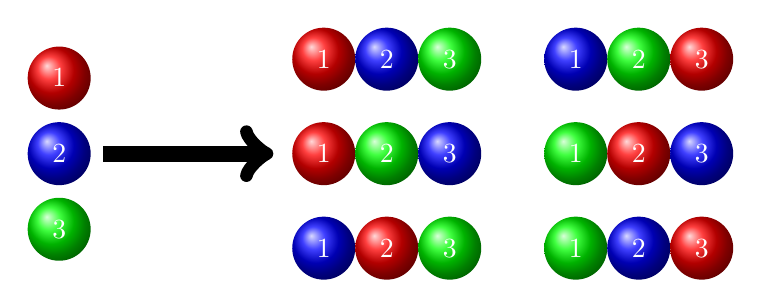
\begin{tikzpicture}[scale=0.8]
\foreach \x / \y / \n in {red/1.2/1, blue/0/2, green/-1.2/3}
 \shade[ball color=\x] (-1.2,\y) circle (0.5cm) node [white] {\n};
 \draw [thick, ->, line width = 0.2cm] (-0.5,0) -- (2.2,0);
\foreach \x / \y / \n in {red/3/1, blue/4/2, green/5/3}
 \shade[ball color=\x] (\y,1.5) circle (0.5cm) node [white] {\n};
   \shade[ball color=red] (3,0) circle (0.5cm) node [white] {1};
 \shade[ball color=green] (4, 0) circle (0.5cm) node [white] {2};
  \shade[ball color=blue] (5, 0) circle (0.5cm) node [white] {3};
   \shade[ball color=blue] (3,-1.5) circle (0.5cm) node [white] {1};
 \shade[ball color=red] (4, -1.5) circle (0.5cm) node [white] {2};
  \shade[ball color=green] (5, -1.5) circle (0.5cm) node [white] {3};
   \shade[ball color=blue] (7,1.5) circle (0.5cm) node [white] {1};
 \shade[ball color=green] (8, 1.5) circle (0.5cm) node [white] {2};
  \shade[ball color=red] (9, 1.5) circle (0.5cm) node [white] {3};
   \shade[ball color=green] (7,0) circle (0.5cm) node [white] {1};
 \shade[ball color=red] (8, 0) circle (0.5cm) node [white] {2};
  \shade[ball color=blue] (9, 0) circle (0.5cm) node [white] {3};
   \shade[ball color=green] (7,-1.5) circle (0.5cm) node [white] {1};
 \shade[ball color=blue] (8, -1.5) circle (0.5cm) node [white] {2};
  \shade[ball color=red] (9, -1.5) circle (0.5cm) node [white] {3};
\end{tikzpicture}
\caption{A permutation of 3 distinct objects.}
\end{figure}
\end{frame}


\begin{frame}[t]
\begin{ex}
How many permutations are there of numbers $123$?
\end{ex}
\begin{sol}
The permutations are 
\[\text{123}, \qquad \text{132}, \qquad, \text{213}, \qquad \text{231}, \qquad \text{312}, \qquad \text{321},\]
which we can search exhaustively using the tree diagram below. Hence, there are 6 permutations. 

\begin{figure}[h!]
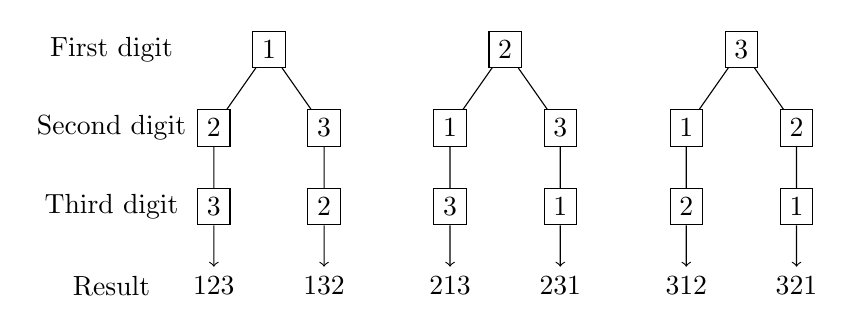
\begin{tikzpicture}[
level distance = 10mm,
level 1/.style={sibling distance=14mm},
]
  \node[rectangle, draw] {1}
    child {node[rectangle, draw] {2}
    	child {node[rectangle, draw] {3}
    		child {node {123}  edge from parent[->]}
    	}
    }
    child {node[rectangle, draw] {3}
    	child {node[rectangle, draw] {2}
    		child {node {132} edge from parent[->]}
    	}
    }
;
  \node[rectangle, draw] at (3,0) {2}
    child {node[rectangle, draw] {1}
    	child {node[rectangle, draw] {3}
    		child {node {213}  edge from parent[->]}
    	}
    }
    child {node[rectangle, draw] {3}
    	child {node[rectangle, draw] {1}
    		child {node {231} edge from parent[->]}
    	}
    }
;
  \node[rectangle, draw] at (6,0) {3}
    child {node[rectangle, draw] {1}
    	child {node[rectangle, draw] {2}
    		child {node {312}  edge from parent[->]}
    	}
    }
    child {node[rectangle, draw] {2}
    	child {node[rectangle, draw] {1}
    		child {node {321} edge from parent[->]}
    	}
    }
;
\node at (-2,0) {First digit};
\node at (-2,-1) {Second digit};
\node at (-2,-2) {Third digit};
\node at (-2,-3) {Result};
\end{tikzpicture}
\end{figure}
\end{sol}
\end{frame}


\begin{frame}[t]
\begin{ex}
How many permutations are there of 2 letters from ABCD?
\end{ex}
\begin{sol}
The permutations are 
\begin{table}[h!]
\centering
\begin{tabular}{cccccc}
AB & AC & AD & BA & BC & BD \\
CA & CB & CD & DA & DB & DC
\end{tabular}
\end{table}
Hence, there are 12 permutations, as illustrated in the tree diagram below.

\begin{figure}[h!]
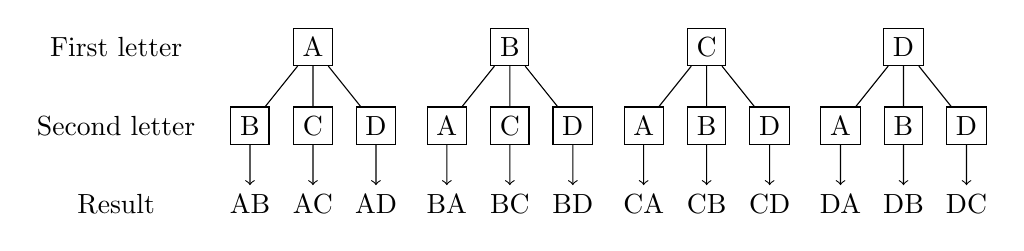
\begin{tikzpicture}[
level distance = 10mm,
sibling distance = 8mm
]
  \node[rectangle, draw] {A}
    	child {node[rectangle, draw] {B}
    		child {node {AB}  edge from parent[->]}
    	}
        	child {node[rectangle, draw] {C}
    		child {node {AC}  edge from parent[->]}
    	}
        	child {node[rectangle, draw] {D}
    		child {node {AD}  edge from parent[->]}
    	}
;  
	\node[rectangle, draw] at (2.5,0) {B}
    	child {node[rectangle, draw] {A}
    		child {node {BA}  edge from parent[->]}
    	}
        	child {node[rectangle, draw] {C}
    		child {node {BC}  edge from parent[->]}
    	}
        	child {node[rectangle, draw] {D}
    		child {node {BD}  edge from parent[->]}
    	}
;
  \node[rectangle, draw] at (5,0) {C}
    	child {node[rectangle, draw] {A}
    		child {node {CA}  edge from parent[->]}
    	}
        	child {node[rectangle, draw] {B}
    		child {node {CB}  edge from parent[->]}
    	}
        	child {node[rectangle, draw] {D}
    		child {node {CD}  edge from parent[->]}
    	}
;
 \node[rectangle, draw] at (7.5,0) {D}
    	child {node[rectangle, draw] {A}
    		child {node {DA}  edge from parent[->]}
    	}
        	child {node[rectangle, draw] {B}
    		child {node {DB}  edge from parent[->]}
    	}
        	child {node[rectangle, draw] {D}
    		child {node {DC}  edge from parent[->]}
    	}
;
\node at (-2.5,0) {First letter};
\node at (-2.5,-1) {Second letter};
\node at (-2.5,-2) {Result};
\end{tikzpicture}
\end{figure}
\end{sol}
\end{frame}


\begin{frame}[t]
\begin{ex}
How many permutations are there of 3 letters in the English alphabet?
\end{ex}
\begin{sol}
Listing all permutations is possible, but would be a waste of paper. Instead, we use a rule of product to help counting. There are three arrangements to make.
\begin{itemize}
\item Choosing the first letter: there are 26 ways.
\item Choosing the second letter: there are 25 ways left, as one of the letters has already been chosen.
\item Choosing the third letter: there are 24 ways left, as two of them have already been chosen.
\end{itemize}
Since we have to make all three arrangements, then by the rule of product there are $26 \times 25 \times 24 = 15,600$ permutations.
\end{sol}
\end{frame}

\begin{frame}[t]
\frametitle{Generalization}
\begin{slide}
We can generalize the procedure in the previous example as follows. If there are $n$ objects and we order $r$ of them, then there are $r$ arrangements to make.
\begin{itemize}
\item Choosing the first object: there are $n$ ways.
\item Choosing the second object: there are $n-1$ ways, as you cannot choose the first object again.
\item Choosing the third object: there are $n-2$ ways, as you cannot choose the first two object.
\item $\vdots$
\item Choosing the $r$-th object: there are $n-(r-1) = n-r+1$ ways, as you cannot choose the first $r-1$ objects.
\end{itemize}
Hence, by the rule of product, we can multiply all the numbers from each arrangement to get the following theorem.
\end{slide}
\end{frame}

\begin{frame}{}
\begin{figure}[h!]
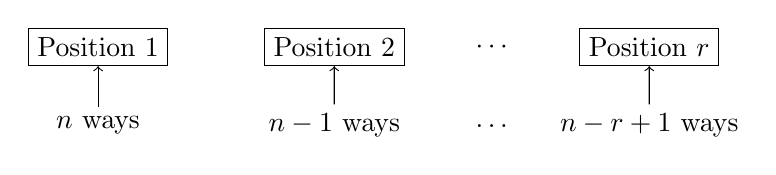
\begin{tikzpicture}[
level distance = 10mm,
level 1/.style={sibling distance=14mm},
]
  \node[rectangle, draw] {Position 1}
    child {node {$n$ ways} edge from parent [<-]};
  \node[rectangle, draw] at (3,0) {Position 2}
    child {node {$n-1$ ways} edge from parent [<-]};    
  \node at (5,0) {$\cdots$}
    child {node {$\ldots$} edge from parent [draw = none]};
   \node[rectangle, draw] at (7,0) {Position $r$}
    child {node {$n-r+1$ ways} edge from parent [<-]};
\end{tikzpicture}
\caption{Counting the number of permutations of $r$ objects from $n$ distinct objects.}
\end{figure}
\end{frame}

\begin{frame}
\frametitle{The Formula for Permutation}
\begin{thm}{}{}
The number of permutations of $n$ objects taken $r$ at a time is denoted 
\[ P(n,r) = n \times  (n-1) \times (n-2) \times \ldots \times (n-r+1) \]
\end{thm}
\end{frame}


\begin{frame}[t]
\begin{ex}
Suppose that 4 people are are to be randomly chosen out of 10 people who agreed to be interviewed in a market survey. How many permutations are there?
\end{ex}
\begin{sol}
The four people are to be assigned to four interviewers, so the order matters. Thus, the number of permutations is 
\[P(10,4) = 10\cdot 9 \cdot 8 \cdot 7 = 5040.\]
\end{sol}
\end{frame}

\begin{frame}{Properties of Permutation (1/2)}
\begin{prop}{}{}
\begin{itemize}
\item $P(n, 0) = 1$: \begin{slide}There is exactly 1 permutation with 0 objects.\end{slide}
\item $P(n,1) = n$: \begin{slide}A permutation of 1 object is simply picking one object.\end{slide}
\item $P(n,n) = n!$: \begin{slide}The number of permutation of all $n$ objects is simply the definition of factorial.\end{slide}
\end{itemize}
\end{prop}
\end{frame}

\begin{frame}{Properties of Permutation (2/2)}
\begin{prop}{}{}
\begin{itemize}
\item $P(n,r) = \frac{n!}{(n-r)!}$: \begin{slide} We can use the factorial to rewrite  as
\begin{eq*}
&&P(n,r) \\
&=&  n \times  (n-1) \times \ldots \times (n-r+1)  \\
&=& \frac{n \times  (n-1) \times \ldots \times (n-r+1) \times \green{ (n-r) \times \ldots \times 2 \times 1}}{\green{(n-r) \times (n-r-1) \times \ldots \times 2 \times 1}} \\
&=& \frac{n!}{(n-r)!}
\end{eq*}
\end{slide}
\end{itemize}
\end{prop}
\end{frame}


%%%%%%%%%%%%%
\section{Combination}
\frame{\sectionpage}
%%%%%%%%%%%%%

\begin{frame}
\frametitle{3. Combination}
\begin{defn}{}{}
\textbf{Combinations} are the possible selections of $r$ items from a group of $n$ items \textit{regardless of the order} of selection. To put it in another way, they are the possible sets of $n$ items. 
\end{defn}
\begin{figure}[h!]
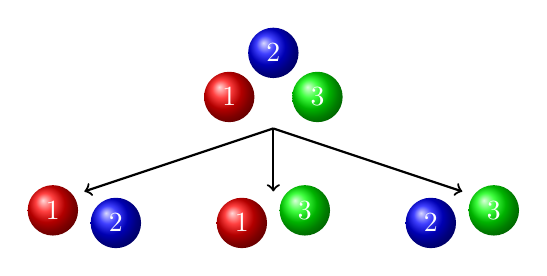
\begin{tikzpicture}[scale =0.8]
 \shade[ball color=red] (-0.7,0) circle (0.4cm) node [white] {1};
 \shade[ball color=blue] (0,0.7) circle (0.4cm) node [white] {2};
 \shade[ball color=green] (0.7,0) circle (0.4cm) node [white] {3};
 \draw [thick, ->] (0,-0.5) -- (-3,-1.5);
 \shade[ball color=red] (-3.5,-1.8) circle (0.4cm) node [white] {1};
 \shade[ball color=blue] (-2.5,-2) circle (0.4cm) node [white] {2};
  \draw [thick, ->] (0,-0.5) -- (0,-1.5);
 \shade[ball color=red] (-0.5,-2) circle (0.4cm) node [white] {1};
 \shade[ball color=green] (0.5,-1.8) circle (0.4cm) node [white] {3};
   \draw [thick, ->] (0,-0.5) -- (3,-1.5);
    \shade[ball color=blue] (2.5,-2) circle (0.4cm) node [white] {2};
 \shade[ball color=green] (3.5,-1.8) circle (0.4cm) node [white] {3};
\end{tikzpicture}
\caption{A combination of 2 objects from 3 distinct objects.}
\end{figure}
\end{frame}


\begin{frame}[t]
\begin{ex}
How many combinations of 2 letters are there of letters $ABC$?
\end{ex}
\begin{sol}
The combinations are 
\[\{\text{A,B}\} \qquad \{\text{B, C}\} \qquad \{\text{A, C}\}.\]
Hence, there are 3 combinations of 2 letters.
\end{sol}
\end{frame}


\begin{frame}[t]
\begin{ex}
How many combinations are there of 3 letters from ABCDE?
\end{ex}
\begin{sol}
The combinations are
\begin{table}[h!]
\centering
\begin{tabular}{CCCCC}
\{\text{A,B,C}\} & \{\text{A,B,D}\} & \{\text{A,B,E}\} & \{ \text{A,C,D} \} & \{ \text{A,C,E} \} \\
\{\text{A,D,E}\} & \{\text{B,C,D}\} & \{\text{B,C,E}\} & \{\text{B,D,E}\} & \{\text{C,D,E}\}
\end{tabular}
\end{table}
Hence, there are 10 combinations.
\end{sol}
\end{frame}

\begin{frame}
\begin{thm}{}{}
The number of combinations is denoted by
\[ C(n,r) = \frac{n!}{r! (n-r)!}.\]
As this notation is very frequently used, we slightly abbreviate $C(n,r) = { n \choose r}$.
\end{thm}
\end{frame}


\begin{frame}[t]
\begin{ex}
How many different flush hands are there in the standard 5-card poker?
\end{ex}
\begin{sol}
We first choose which suit $\clubsuit, \vardiamondsuit, \spadesuit, \varheartsuit$ to form, in which there are 4 ways. Then, we choose 5 out of 13 possible values, in which there are $\ch{13}{5} = \frac{13 \times 12 \times 11 \times 10 \times 9}{5 \times 4 \times 3 \times 2 \times 1} = 1287$ ways. Since choosing a suit and choosing card values are two arrangements, we use the rule of product to get
\[ \ch{13}{5} \times 4 = 5148\]
\end{sol}
\end{frame}

\begin{frame}
\frametitle{Properties}
\begin{prop}{}{}
\begin{enumerate}
\item $\ch{n}{0} = \ch{n}{n} = 1$. \begin{slide}This explains that there is only one way to choose nothing. There is also only one way to choose everything.\end{slide}
\item $\ch{n}{1} = n$. \begin{slide}A combination of 1 object is the same as selecting 1 object.\end{slide}
\end{enumerate}
\end{prop}
\end{frame}



\begin{frame}
\frametitle{Properties}
\begin{prop}{}{}
\begin{enumerate}
\item $\ch{n}{k} = \ch{n}{n-k}$. \begin{slide}This can be proved numerically 
\[ \ch{n}{k} = \frac{n!}{k! (n-k)!} = \frac{n!}{(n-k)! (n- (n-k))!} = \ch{n}{n-k}.\]
or, better yet, combinatorially. If there are $n$ distinct objects, then the number of ways to choose $k$ objects is the same as the number of ways to discard $n-k$ objects.\end{slide}
\end{enumerate}
\end{prop}
\end{frame}

\begin{frame}
\begin{prop}{}{}
\begin{enumerate} \setcounter{enumi}{2}
\item $P(n,r) = C(n,r) \times r!$. \begin{slide} This says that you can get a permutation by first getting a combination, and then order those $r$ objects. This proves the formula
\[ C(n,r) = \frac{P(n,r)}{r!} = \frac{n!/(n-r)!}{r!} = \frac{n!}{(n-r)!r!}. \] \end{slide}
\end{enumerate}
\end{prop}
\end{frame}

